%sec1: comment trouve-t-on les surprises
%sec2: surprises and sale dynamics
%sec3: precision of the prior

%Sales of movies with positive surprise and sales of movies with negative surprise should diverge over time. To test this, we need to regress the log of sales on time and the interaction between time and surprise. If the coefficient of the interaction between time and surprise is significantly positive, then the sales of movies with positive surprise decrease slower than the sale of movies with negative surprise. If our results are consistent with those of Moretti, we should find that controlling for advertising, critic reviews and other variables does not affect significantly the results.

% The effect of a surprise should be lower for movies with a more precise prior. To test this, we augment the previous regression equation with the interaction of time and the precision of the prior and the interaction of time, precision of the prior and surprise of the movie (whose coefficient is predicted to be negative). The precision of the prior can be a dummy for sequels (sequels are assumed to have a more precise prior) or can be measured by the variance of the first week surprise for movies of the same genre.

\subsection{Identification of the surprises}

Surprises consist in the residuals of the regression of the log-number of sales in the first week on the log-number of screens available (opened by theaters). This definition of surprises holds because we suppose that theaters are profit-maximizing agents and make use of all the available information to predict the success of a movie. If this definition is correct, we should expect log-number of screens opened by theaters first week to be a good indicator of knowledge available on the movie quality before it is released. In the Table \ref{part2.1_tab1} we reproduce Moretti's regression of \textit{log\_sales\_first\_we} on \textit{log\_screens\_first\_week}. Each column is the result of the regression when we control with some variables (film genre, rating available, cost, distributor, weekday, month, week, year). The fact that adding control variables doesn't change the robustness of the regression proves Moretti's point which is that theaters take into account these factors when deciding their number of available screens. 

\begin{table}[!htbp] \centering 
	\caption{Regression of first-weekend sales on number of screens} 
	\label{part2.1_tab1} 
	\begin{tabular}{@{\extracolsep{5pt}}lccccccc} 
		\\[-1.8ex]\hline 
		\hline \\[-1.8ex] 
		& \multicolumn{7}{c}{\textit{Dependent variable:}} \\ 
		\cline{2-8} 
		\\[-1.8ex] & \multicolumn{7}{c}{log\_sales\_first\_we} \\ 
		\\[-1.8ex] & (1) & (2) & (3) & (4) & (5) & (6) & (7)\\ 
		\hline \\[-1.8ex] 
		log\_screens\_first\_week & 0.893$^{***}$ & 0.896$^{***}$ & 0.883$^{***}$ & 0.871$^{***}$ & 0.803$^{***}$ & 0.806$^{***}$ & 0.813$^{***}$ \\ 
		& (0.004) & (0.005) & (0.005) & (0.005) & (0.006) & (0.006) & (0.006) \\ 
		& & & & & & & \\ 
		\hline \\[-1.8ex] 
		R$^{2}$ & 0.907 & 0.909 & 0.910 & 0.912 & 0.932 & 0.936 & 0.938 \\ 
		Adjusted R$^{2}$ & 0.907 & 0.908 & 0.910 & 0.912 & 0.928 & 0.931 & 0.933 \\ 
		\hline 
		\hline \\[-1.8ex] 
		\textit{Note:}  & \multicolumn{7}{r}{$^{*}$p$<$0.1; $^{**}$p$<$0.05; $^{***}$p$<$0.01} \\ 
	\end{tabular} 
\end{table} 
In fact, theaters perform more than what we could do using all the data available in the data set. Regressing first week-end sales on our control variables gives us a R\textsuperscript{2} of .7, which is smaller than .9 performed by theaters only.
\todo{is this useful?}
\todo{nope, you only need the significativity of the coefficient}
\begin{table}[!htbp] \centering 
	\caption{Regression of first-weekend sales on control variables} 
	\label{part2.1_tab2} 
	\begin{tabular}{@{\extracolsep{5pt}}lc} 
		\\[-1.8ex]\hline 
		\hline \\[-1.8ex] 
		& \multicolumn{1}{c}{\textit{Dependent variable:}} \\ 
		\cline{2-2} 
		\\[-1.8ex] & log\_sales\_first\_we \\ 
		\hline \\[-1.8ex] 
		\hline \\[-1.8ex] 
		Observations & 4,992 \\ 
		R$^{2}$ & 0.699 \\ 
		Adjusted R$^{2}$ & 0.674 \\ 
		\hline 
		\hline \\[-1.8ex] 
		\textit{Note:}  & \multicolumn{1}{r}{$^{*}$p$<$0.1; $^{**}$p$<$0.05; $^{***}$p$<$0.01} \\ 
	\end{tabular} 
\end{table}
\paragraph*{}
We have performed the same kind of regression on France data from 2004 to 2008 and find quite similar results (Table \ref{part2.1_tab3} for France data and Table \ref{part2.1_tab4} for Paris data only\footnote{Data available for Paris are richer of 600 movies than France.}).
\begin{table}[!htbp] \centering 
	\caption{Regression of first-week entries on number of screens for France} 
	\label{part2.1_tab3} 
	\begin{tabular}{@{\extracolsep{5pt}}lccccccc} 
		\\[-1.8ex]\hline 
		\hline \\[-1.8ex] 
		& \multicolumn{7}{c}{\textit{Dependent variable:}} \\ 
		\cline{2-8} 
		\\[-1.8ex] & \multicolumn{7}{c}{log\_entree\_fr} \\ 
		\\[-1.8ex] & (1) & (2) & (3) & (4) & (5) & (6) & (7)\\ 
		\hline \\[-1.8ex] 
		log\_seance\_fr & 1.208$^{***}$ & 1.237$^{***}$ & 1.237$^{***}$ & 1.279$^{***}$ & 1.282$^{***}$ & 1.287$^{***}$ & 1.196$^{***}$ \\ 
		& (0.009) & (0.010) & (0.010) & (0.014) & (0.014) & (0.014) & (0.014) \\ 
		& & & & & & & \\ 
		\hline \\[-1.8ex] 
		Observations & 2,046 & 2,046 & 2,046 & 2,046 & 2,046 & 2,046 & 2,046 \\ 
		R$^{2}$ & 0.893 & 0.899 & 0.900 & 0.917 & 0.924 & 0.925 & 0.943 \\ 
		Adjusted R$^{2}$ & 0.893 & 0.898 & 0.898 & 0.910 & 0.915 & 0.916 & 0.935 \\ 
		\hline 
		\hline \\[-1.8ex] 
		\textit{Note:}  & \multicolumn{7}{r}{$^{*}$p$<$0.1; $^{**}$p$<$0.05; $^{***}$p$<$0.01} \\ 
	\end{tabular} 
\end{table} 

\begin{table}[!htbp] \centering 
	\caption{Regression of first-week entries on number of screens for Paris only} 
	\label{part2.1_tab4} 
	\begin{tabular}{@{\extracolsep{5pt}}lccccccc} 
		\\[-1.8ex]\hline 
		\hline \\[-1.8ex] 
		& \multicolumn{7}{c}{\textit{Dependent variable:}} \\ 
		\cline{2-8} 
		\\[-1.8ex] & \multicolumn{7}{c}{log\_entree\_paris} \\ 
		\\[-1.8ex] & (1) & (2) & (3) & (4) & (5) & (6) & (7)\\ 
		\hline \\[-1.8ex] 
		log\_seance\_paris & 1.342$^{***}$ & 1.336$^{***}$ & 1.337$^{***}$ & 1.281$^{***}$ & 1.281$^{***}$ & 1.284$^{***}$ & 1.152$^{***}$ \\ 
		& (0.010) & (0.011) & (0.011) & (0.014) & (0.014) & (0.014) & (0.014) \\ 
		& & & & & & & \\ 
		\hline \\[-1.8ex] 
		Observations & 2,701 & 2,701 & 2,701 & 2,701 & 2,701 & 2,701 & 2,701 \\ 
		R$^{2}$ & 0.875 & 0.880 & 0.881 & 0.901 & 0.908 & 0.909 & 0.927 \\ 
		Adjusted R$^{2}$ & 0.875 & 0.879 & 0.880 & 0.892 & 0.897 & 0.898 & 0.918 \\ 
		\hline 
		\hline \\[-1.8ex] 
		\textit{Note:}  & \multicolumn{7}{r}{$^{*}$p$<$0.1; $^{**}$p$<$0.05; $^{***}$p$<$0.01} \\ 
	\end{tabular} 
\end{table} 
\begin{figure}\centering
	\caption{We find the same graph as Moretti}
	\label{part2.1_plot_moretti}
	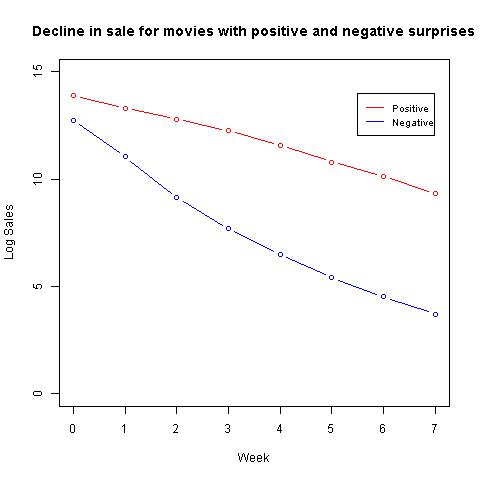
\includegraphics[scale=0.5]{plot_moretti.png}
\end{figure}
\begin{figure}\centering
	\label{part2.1_plot_fr}
	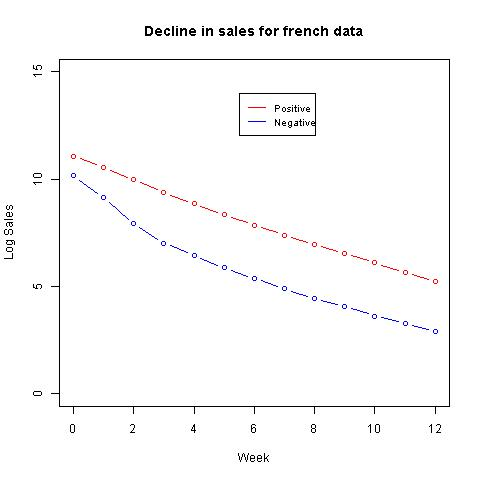
\includegraphics[scale=0.5]{plot_fr.png}
\end{figure}
\begin{figure}\centering
	\label{part2.1_plot_paris}
	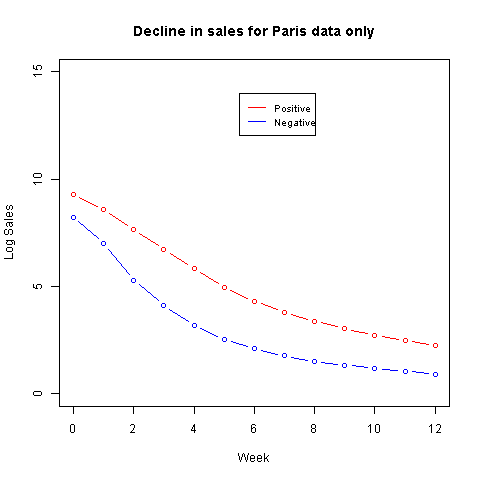
\includegraphics[scale=0.5]{plot_paris_only.png}
\end{figure}

% Table created by stargazer v.5.2 by Marek Hlavac, Harvard University. E-mail: hlavac at fas.harvard.edu
% Date and time: Wed, Feb 28, 2018 - 14:38:13
\begin{table}[!htbp] \centering 
	\caption{Decline in box-office sales by opening week surprise} 
	\label{} 
	\begin{tabular}{@{\extracolsep{5pt}}lcccc} 
		\\[-1.8ex]\hline 
		\hline \\[-1.8ex] 
		& \multicolumn{4}{c}{\textit{Dependent variable:}} \\ 
		\cline{2-5} 
		\\[-1.8ex] & \multicolumn{4}{c}{log\_sales} \\ 
		\\[-1.8ex] & (1) & (2) & (3) & (4)\\ 
		\hline \\[-1.8ex] 
		t & $-$0.952$^{***}$ & $-$0.952$^{***}$ & $-$1.289$^{***}$ &  \\ 
		& (0.007) & (0.006) & (0.009) &  \\ 
		& & & & \\ 
		t:surprise &  & 0.475$^{***}$ &  &  \\ 
		&  & (0.009) &  &  \\ 
		& & & & \\ 
		t:positive\_surprise &  &  & 0.640$^{***}$ &  \\ 
		&  &  & (0.013) &  \\ 
		& & & & \\ 
		I(t \textasteriskcentered  bottom\_surprise) &  &  &  & $-$1.353$^{***}$ \\ 
		&  &  &  & (0.011) \\ 
		& & & & \\ 
		I(t \textasteriskcentered  middle\_surprise) &  &  &  & $-$1.011$^{***}$ \\ 
		&  &  &  & (0.011) \\ 
		& & & & \\ 
		I(t \textasteriskcentered  top\_surprise) &  &  &  & $-$0.491$^{***}$ \\ 
		&  &  &  & (0.011) \\ 
		& & & & \\ 
		\hline \\[-1.8ex] 
		Observations & 39,936 & 39,936 & 39,936 & 39,936 \\ 
		R$^{2}$ & 0.772 & 0.788 & 0.787 & 0.790 \\ 
		Adjusted R$^{2}$ & 0.739 & 0.758 & 0.756 & 0.760 \\ 
		\hline 
		\hline \\[-1.8ex] 
		\textit{Note:}  & \multicolumn{4}{r}{$^{*}$p$<$0.1; $^{**}$p$<$0.05; $^{***}$p$<$0.01} \\ 
	\end{tabular} 
\end{table} 

% Table created by stargazer v.5.2 by Marek Hlavac, Harvard University. E-mail: hlavac at fas.harvard.edu
% Date and time: Wed, Feb 28, 2018 - 14:38:13
\begin{table}[!htbp] \centering 
	\caption{Precision of the prior} 
	\label{} 
	\begin{tabular}{@{\extracolsep{5pt}}lcc} 
		\\[-1.8ex]\hline 
		\hline \\[-1.8ex] 
		& \multicolumn{2}{c}{\textit{Dependent variable:}} \\ 
		\cline{2-3} 
		\\[-1.8ex] & \multicolumn{2}{c}{log\_sales} \\ 
		\\[-1.8ex] & (1) & (2)\\ 
		\hline \\[-1.8ex] 
		t & $-$1.291$^{***}$ & $-$1.267$^{***}$ \\ 
		& (0.010) & (0.087) \\ 
		& & \\ 
		t:positive\_surprise & 0.654$^{***}$ & $-$0.061 \\ 
		& (0.013) & (0.121) \\ 
		& & \\ 
		t:sequel & 0.037 &  \\ 
		& (0.038) &  \\ 
		& & \\ 
		t:positive\_surpriseTRUE:sequel & $-$0.225$^{***}$ &  \\ 
		& (0.053) &  \\ 
		& & \\ 
		t:var\_surprise &  & $-$0.045 \\ 
		&  & (0.174) \\ 
		& & \\ 
		t:positive\_surpriseTRUE:var\_surprise &  & 1.416$^{***}$ \\ 
		&  & (0.243) \\ 
		& & \\ 
		\hline \\[-1.8ex] 
		Observations & 39,936 & 39,936 \\ 
		R$^{2}$ & 0.787 & 0.787 \\ 
		Adjusted R$^{2}$ & 0.756 & 0.757 \\ 
		\hline 
		\hline \\[-1.8ex] 
		\textit{Note:}  & \multicolumn{2}{r}{$^{*}$p$<$0.1; $^{**}$p$<$0.05; $^{***}$p$<$0.01} \\ 
	\end{tabular} 
\end{table} 

FRANCE

% Table created by stargazer v.5.2 by Marek Hlavac, Harvard University. E-mail: hlavac at fas.harvard.edu
% Date and time: Wed, Feb 28, 2018 - 14:27:55
\begin{table}[!htbp] \centering 
	\caption{Decline in box-office sales by opening week surprise} 
	\label{} 
	\begin{tabular}{@{\extracolsep{5pt}}lcccc} 
		\\[-1.8ex]\hline 
		\hline \\[-1.8ex] 
		& \multicolumn{4}{c}{\textit{Dependent variable:}} \\ 
		\cline{2-5} 
		\\[-1.8ex] & \multicolumn{4}{c}{log\_entree\_fr} \\ 
		\\[-1.8ex] & (1) & (2) & (3) & (4)\\ 
		\hline \\[-1.8ex] 
		t & $-$0.526$^{***}$ & $-$0.526$^{***}$ & $-$0.571$^{***}$ &  \\ 
		& (0.002) & (0.002) & (0.003) &  \\ 
		& & & & \\ 
		t:surprise &  & 0.076$^{***}$ &  &  \\ 
		&  & (0.004) &  &  \\ 
		& & & & \\ 
		t:positive\_surprise &  &  & 0.087$^{***}$ &  \\ 
		&  &  & (0.004) &  \\ 
		& & & & \\ 
		t:bottom\_surpriseFALSE &  &  &  & $-$0.459$^{***}$ \\ 
		&  &  &  & (0.004) \\ 
		& & & & \\ 
		t:bottom\_surprise &  &  &  & $-$0.574$^{***}$ \\ 
		&  &  &  & (0.004) \\ 
		& & & & \\ 
		t:middle\_surprise &  &  &  & $-$0.088$^{***}$ \\ 
		&  &  &  & (0.005) \\ 
		& & & & \\ 
		\hline \\[-1.8ex] 
		Observations & 26,598 & 26,598 & 26,598 & 26,598 \\ 
		R$^{2}$ & 0.851 & 0.853 & 0.853 & 0.854 \\ 
		Adjusted R$^{2}$ & 0.838 & 0.841 & 0.841 & 0.841 \\ 
		\hline 
		\hline \\[-1.8ex] 
		\textit{Note:}  & \multicolumn{4}{r}{$^{*}$p$<$0.1; $^{**}$p$<$0.05; $^{***}$p$<$0.01} \\ 
	\end{tabular} 
\end{table} 

% Table created by stargazer v.5.2 by Marek Hlavac, Harvard University. E-mail: hlavac at fas.harvard.edu
% Date and time: Wed, Feb 28, 2018 - 14:27:56
\begin{table}[!htbp] \centering 
	\caption{Precision of the prior} 
	\label{} 
	\begin{tabular}{@{\extracolsep{5pt}}lccc} 
		\\[-1.8ex]\hline 
		\hline \\[-1.8ex] 
		& \multicolumn{3}{c}{\textit{Dependent variable:}} \\ 
		\cline{2-4} 
		\\[-1.8ex] & \multicolumn{3}{c}{log\_entree\_fr} \\ 
		\\[-1.8ex] & (1) & (2) & (3)\\ 
		\hline \\[-1.8ex] 
		t & $-$0.570$^{***}$ & $-$0.698$^{***}$ & $-$0.678$^{***}$ \\ 
		& (0.003) & (0.013) & (0.004) \\ 
		& & & \\ 
		t:positive\_surprise & 0.105$^{***}$ & 0.109$^{***}$ & 0.009 \\ 
		& (0.005) & (0.018) & (0.006) \\ 
		& & & \\ 
		t:saga & $-$0.027 &  &  \\ 
		& (0.016) &  &  \\ 
		& & & \\ 
		t:positive\_surpriseTRUE:saga & $-$0.145$^{***}$ &  &  \\ 
		& (0.019) &  &  \\ 
		& & & \\ 
		t:var\_surprise &  & 0.370$^{***}$ &  \\ 
		&  & (0.035) &  \\ 
		& & & \\ 
		t:positive\_surpriseTRUE:var\_surprise &  & $-$0.062 &  \\ 
		&  & (0.050) &  \\ 
		& & & \\ 
		t:art\_essai &  &  & 0.259$^{***}$ \\ 
		&  &  & (0.006) \\ 
		& & & \\ 
		t:positive\_surpriseTRUE:art\_essai &  &  & 0.066$^{***}$ \\ 
		&  &  & (0.008) \\ 
		& & & \\ 
		\hline \\[-1.8ex] 
		Observations & 26,598 & 26,546 & 26,598 \\ 
		R$^{2}$ & 0.855 & 0.854 & 0.880 \\ 
		Adjusted R$^{2}$ & 0.843 & 0.842 & 0.870 \\ 
		\hline 
		\hline \\[-1.8ex] 
		\textit{Note:}  & \multicolumn{3}{r}{$^{*}$p$<$0.1; $^{**}$p$<$0.05; $^{***}$p$<$0.01} \\ 
	\end{tabular} 
\end{table} 

PARIS

% Table created by stargazer v.5.2 by Marek Hlavac, Harvard University. E-mail: hlavac at fas.harvard.edu
% Date and time: Wed, Feb 28, 2018 - 14:37:16
\begin{table}[!htbp] \centering 
	\caption{Decline in box-office sales by opening week surprise} 
	\label{} 
	\begin{tabular}{@{\extracolsep{5pt}}lcccc} 
		\\[-1.8ex]\hline 
		\hline \\[-1.8ex] 
		& \multicolumn{4}{c}{\textit{Dependent variable:}} \\ 
		\cline{2-5} 
		\\[-1.8ex] & \multicolumn{4}{c}{log\_entree\_paris} \\ 
		\\[-1.8ex] & (1) & (2) & (3) & (4)\\ 
		\hline \\[-1.8ex] 
		t & $-$0.583$^{***}$ & $-$0.583$^{***}$ & $-$0.564$^{***}$ &  \\ 
		& (0.002) & (0.002) & (0.003) &  \\ 
		& & & & \\ 
		t:surprise &  & $-$0.032$^{***}$ &  &  \\ 
		&  & (0.004) &  &  \\ 
		& & & & \\ 
		t:positive\_surprise &  &  & $-$0.039$^{***}$ &  \\ 
		&  &  & (0.005) &  \\ 
		& & & & \\ 
		t:bottom\_surpriseFALSE &  &  &  & $-$0.594$^{***}$ \\ 
		&  &  &  & (0.004) \\ 
		& & & & \\ 
		t:bottom\_surprise &  &  &  & $-$0.541$^{***}$ \\ 
		&  &  &  & (0.004) \\ 
		& & & & \\ 
		t:middle\_surprise &  &  &  & $-$0.021$^{***}$ \\ 
		&  &  &  & (0.006) \\ 
		& & & & \\ 
		\hline \\[-1.8ex] 
		Observations & 35,113 & 35,113 & 35,113 & 35,113 \\ 
		R$^{2}$ & 0.810 & 0.810 & 0.810 & 0.811 \\ 
		Adjusted R$^{2}$ & 0.794 & 0.794 & 0.794 & 0.795 \\ 
		\hline 
		\hline \\[-1.8ex] 
		\textit{Note:}  & \multicolumn{4}{r}{$^{*}$p$<$0.1; $^{**}$p$<$0.05; $^{***}$p$<$0.01} \\ 
	\end{tabular} 
\end{table} 

% Table created by stargazer v.5.2 by Marek Hlavac, Harvard University. E-mail: hlavac at fas.harvard.edu
% Date and time: Wed, Feb 28, 2018 - 14:37:16
\begin{table}[!htbp] \centering 
	\caption{Precision of the prior} 
	\label{} 
	\begin{tabular}{@{\extracolsep{5pt}}lccc} 
		\\[-1.8ex]\hline 
		\hline \\[-1.8ex] 
		& \multicolumn{3}{c}{\textit{Dependent variable:}} \\ 
		\cline{2-4} 
		\\[-1.8ex] & \multicolumn{3}{c}{log\_entree\_paris} \\ 
		\\[-1.8ex] & (1) & (2) & (3)\\ 
		\hline \\[-1.8ex] 
		t & $-$0.560$^{***}$ & $-$0.772$^{***}$ & $-$0.616$^{***}$ \\ 
		& (0.003) & (0.017) & (0.005) \\ 
		& & & \\ 
		t:positive\_surprise & $-$0.030$^{***}$ & $-$0.213$^{***}$ & $-$0.126$^{***}$ \\ 
		& (0.005) & (0.024) & (0.007) \\ 
		& & & \\ 
		t:saga & $-$0.118$^{***}$ &  &  \\ 
		& (0.017) &  &  \\ 
		& & & \\ 
		t:positive\_surpriseTRUE:saga & $-$0.022 &  &  \\ 
		& (0.020) &  &  \\ 
		& & & \\ 
		t:var\_surprise &  & 0.576$^{***}$ &  \\ 
		&  & (0.045) &  \\ 
		& & & \\ 
		t:positive\_surpriseTRUE:var\_surprise &  & 0.480$^{***}$ &  \\ 
		&  & (0.065) &  \\ 
		& & & \\ 
		t:art\_essai &  &  & 0.087$^{***}$ \\ 
		&  &  & (0.006) \\ 
		& & & \\ 
		t:positive\_surpriseTRUE:art\_essai &  &  & 0.156$^{***}$ \\ 
		&  &  & (0.009) \\ 
		& & & \\ 
		\hline \\[-1.8ex] 
		Observations & 35,113 & 35,074 & 35,113 \\ 
		R$^{2}$ & 0.811 & 0.814 & 0.819 \\ 
		Adjusted R$^{2}$ & 0.795 & 0.798 & 0.804 \\ 
		\hline 
		\hline \\[-1.8ex] 
		\textit{Note:}  & \multicolumn{3}{r}{$^{*}$p$<$0.1; $^{**}$p$<$0.05; $^{***}$p$<$0.01} \\ 
	\end{tabular} 
\end{table} 
\subsection{Divergence of the sales}
\subsection{Precision of the prior}
